\documentclass{standalone}
\usepackage{tikz}
\usetikzlibrary{patterns, positioning}


\begin{document}
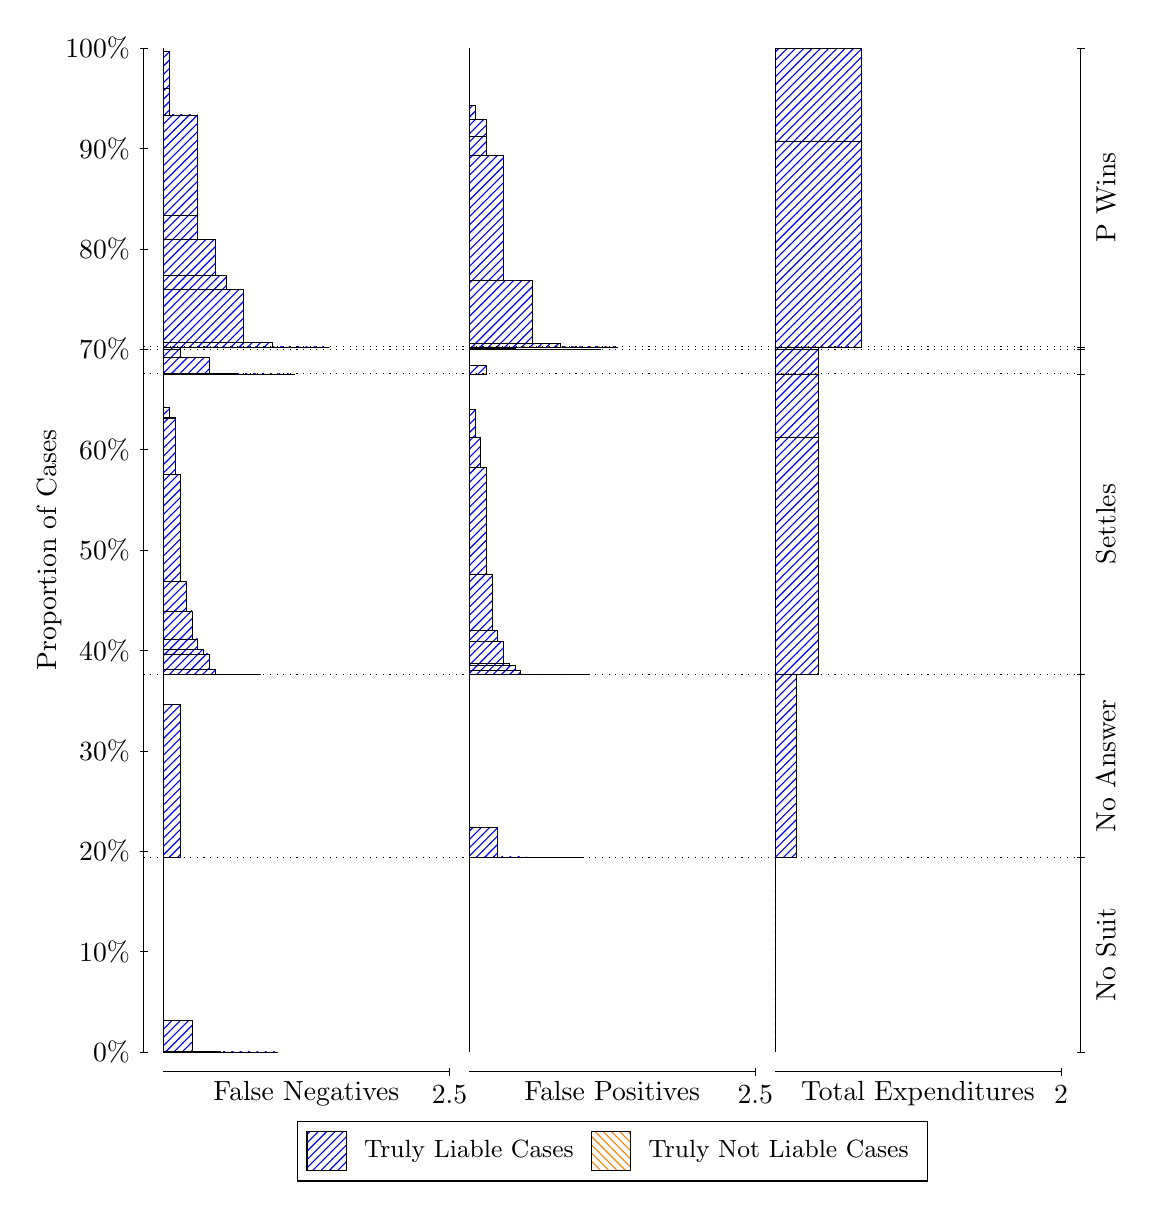
\begin{tikzpicture}
\draw[black, very thin] (1.5,1.75) -- (1.5,14.5);
\node[rotate=90, text=black, anchor=center] at (0.3, 8.125) {Proportion of Cases};
\draw[black, very thin] (1.45,1.75) -- (1.55,1.75);
\node[text=black, anchor=east] at (1.45, 1.75) {0\%};
\draw[black, very thin] (1.45,3.025) -- (1.55,3.025);
\node[text=black, anchor=east] at (1.45, 3.025) {10\%};
\draw[black, very thin] (1.45,4.3) -- (1.55,4.3);
\node[text=black, anchor=east] at (1.45, 4.3) {20\%};
\draw[black, very thin] (1.45,5.575) -- (1.55,5.575);
\node[text=black, anchor=east] at (1.45, 5.575) {30\%};
\draw[black, very thin] (1.45,6.85) -- (1.55,6.85);
\node[text=black, anchor=east] at (1.45, 6.85) {40\%};
\draw[black, very thin] (1.45,8.125) -- (1.55,8.125);
\node[text=black, anchor=east] at (1.45, 8.125) {50\%};
\draw[black, very thin] (1.45,9.4) -- (1.55,9.4);
\node[text=black, anchor=east] at (1.45, 9.4) {60\%};
\draw[black, very thin] (1.45,10.675) -- (1.55,10.675);
\node[text=black, anchor=east] at (1.45, 10.675) {70\%};
\draw[black, very thin] (1.45,11.95) -- (1.55,11.95);
\node[text=black, anchor=east] at (1.45, 11.95) {80\%};
\draw[black, very thin] (1.45,13.225) -- (1.55,13.225);
\node[text=black, anchor=east] at (1.45, 13.225) {90\%};
\draw[black, very thin] (1.45,14.5) -- (1.55,14.5);
\node[text=black, anchor=east] at (1.45, 14.5) {100\%};

\draw[black, very thin] (13.4,1.75) -- (13.4,14.5);
\draw[black, very thin] (13.35,1.75) -- (13.45,1.75);
\node[anchor=west] at (13.35, 1.75) {};
\draw[black, very thin] (13.35,4.2243) -- (13.45,4.2243);
\node[anchor=west] at (13.35, 4.2243) {};
\draw[black, very thin] (13.35,6.5452) -- (13.45,6.5452);
\node[anchor=west] at (13.35, 6.5452) {};
\draw[black, very thin] (13.35,10.363) -- (13.45,10.363);
\node[anchor=west] at (13.35, 10.363) {};
\draw[black, very thin] (13.35,10.677) -- (13.45,10.677);
\node[anchor=west] at (13.35, 10.677) {};
\draw[black, very thin] (13.35,10.704) -- (13.45,10.704);
\node[anchor=west] at (13.35, 10.704) {};
\draw[black, very thin] (13.35,14.5) -- (13.45,14.5);
\node[anchor=west] at (13.35, 14.5) {};

\draw[black, very thin, pattern color=blue, pattern=north east lines] (1.75,1.75) rectangle (3.2033,1.75);
\draw[black, very thin, pattern color=blue, pattern=north east lines] (1.75,1.75) rectangle (2.84,1.75);
\draw[black, very thin, pattern color=blue, pattern=north east lines] (1.75,1.75) rectangle (2.4767,1.7535);
\draw[black, very thin, pattern color=blue, pattern=north east lines] (1.75,1.7535) rectangle (2.1133,2.1551);
\draw[black, very thin, pattern color=orange, pattern=north west lines] (1.75,2.1551) rectangle (1.75,2.1551);
\draw[black, very thin, pattern color=blue, pattern=north east lines] (1.75,2.1551) rectangle (1.75,4.2243);
\draw[black, very thin, pattern color=blue, pattern=north east lines] (1.75,4.2243) rectangle (1.968,6.1651);
\draw[black, very thin, pattern color=orange, pattern=north west lines] (1.75,6.1651) rectangle (1.75,6.1651);
\draw[black, very thin, pattern color=blue, pattern=north east lines] (1.75,6.1651) rectangle (1.75,6.5452);
\draw[black, very thin, pattern color=blue, pattern=north east lines] (1.75,6.5452) rectangle (2.9853,6.5452);
\draw[black, very thin, pattern color=blue, pattern=north east lines] (1.75,6.5452) rectangle (2.84,6.5452);
\draw[black, very thin, pattern color=blue, pattern=north east lines] (1.75,6.5452) rectangle (2.6947,6.5456);
\draw[black, very thin, pattern color=blue, pattern=north east lines] (1.75,6.5456) rectangle (2.622,6.5456);
\draw[black, very thin, pattern color=blue, pattern=north east lines] (1.75,6.5456) rectangle (2.5493,6.546);
\draw[black, very thin, pattern color=blue, pattern=north east lines] (1.75,6.546) rectangle (2.4767,6.5477);
\draw[black, very thin, pattern color=blue, pattern=north east lines] (1.75,6.5477) rectangle (2.404,6.604);
\draw[black, very thin, pattern color=blue, pattern=north east lines] (1.75,6.604) rectangle (2.3313,6.8062);
\draw[black, very thin, pattern color=blue, pattern=north east lines] (1.75,6.8062) rectangle (2.2587,6.8579);
\draw[black, very thin, pattern color=blue, pattern=north east lines] (1.75,6.8579) rectangle (2.186,6.9958);
\draw[black, very thin, pattern color=blue, pattern=north east lines] (1.75,6.9958) rectangle (2.1133,7.3504);
\draw[black, very thin, pattern color=blue, pattern=north east lines] (1.75,7.3504) rectangle (2.0407,7.7294);
\draw[black, very thin, pattern color=blue, pattern=north east lines] (1.75,7.7294) rectangle (1.968,9.0864);
\draw[black, very thin, pattern color=blue, pattern=north east lines] (1.75,9.0864) rectangle (1.8953,9.8014);
\draw[black, very thin, pattern color=blue, pattern=north east lines] (1.75,9.8014) rectangle (1.8953,9.8067);
\draw[black, very thin, pattern color=blue, pattern=north east lines] (1.75,9.8067) rectangle (1.8227,9.9437);
\draw[black, very thin, pattern color=orange, pattern=north west lines] (1.75,9.9437) rectangle (1.75,9.9437);
\draw[black, very thin, pattern color=blue, pattern=north east lines] (1.75,9.9437) rectangle (1.75,10.363);
\draw[black, very thin, pattern color=blue, pattern=north east lines] (1.75,10.363) rectangle (3.4213,10.363);
\draw[black, very thin, pattern color=blue, pattern=north east lines] (1.75,10.363) rectangle (3.058,10.363);
\draw[black, very thin, pattern color=blue, pattern=north east lines] (1.75,10.363) rectangle (2.6947,10.37);
\draw[black, very thin, pattern color=blue, pattern=north east lines] (1.75,10.37) rectangle (2.3313,10.567);
\draw[black, very thin, pattern color=blue, pattern=north east lines] (1.75,10.567) rectangle (1.968,10.677);
\draw[black, very thin, pattern color=orange, pattern=north west lines] (1.75,10.677) rectangle (1.75,10.677);
\draw[black, very thin, pattern color=blue, pattern=north east lines] (1.75,10.677) rectangle (1.968,10.7);
\draw[black, very thin, pattern color=orange, pattern=north west lines] (1.75,10.7) rectangle (1.75,10.7);
\draw[black, very thin, pattern color=blue, pattern=north east lines] (1.75,10.7) rectangle (1.75,10.704);
\draw[black, very thin, pattern color=blue, pattern=north east lines] (1.75,10.704) rectangle (3.8573,10.704);
\draw[black, very thin, pattern color=blue, pattern=north east lines] (1.75,10.704) rectangle (3.494,10.704);
\draw[black, very thin, pattern color=blue, pattern=north east lines] (1.75,10.704) rectangle (3.276,10.704);
\draw[black, very thin, pattern color=blue, pattern=north east lines] (1.75,10.704) rectangle (3.1307,10.766);
\draw[black, very thin, pattern color=blue, pattern=north east lines] (1.75,10.766) rectangle (2.9127,10.766);
\draw[black, very thin, pattern color=blue, pattern=north east lines] (1.75,10.766) rectangle (2.7673,11.434);
\draw[black, very thin, pattern color=blue, pattern=north east lines] (1.75,11.434) rectangle (2.5493,11.615);
\draw[black, very thin, pattern color=blue, pattern=north east lines] (1.75,11.615) rectangle (2.404,12.067);
\draw[black, very thin, pattern color=blue, pattern=north east lines] (1.75,12.067) rectangle (2.186,12.376);
\draw[black, very thin, pattern color=blue, pattern=north east lines] (1.75,12.376) rectangle (2.186,13.652);
\draw[black, very thin, pattern color=blue, pattern=north east lines] (1.75,13.652) rectangle (2.0407,13.652);
\draw[black, very thin, pattern color=blue, pattern=north east lines] (1.75,13.652) rectangle (1.8227,13.991);
\draw[black, very thin, pattern color=blue, pattern=north east lines] (1.75,13.991) rectangle (1.8227,14.454);
\draw[black, very thin, pattern color=orange, pattern=north west lines] (1.75,14.454) rectangle (1.75,14.454);
\draw[black, very thin, pattern color=blue, pattern=north east lines] (1.75,14.454) rectangle (1.75,14.5);
\draw[black, very thin, pattern color=orange, pattern=north west lines] (5.6333,1.75) rectangle (5.6333,1.75);
\draw[black, very thin, pattern color=blue, pattern=north east lines] (5.6333,1.75) rectangle (5.6333,4.2243);
\draw[black, very thin, pattern color=orange, pattern=north west lines] (5.6333,4.2243) rectangle (7.0867,4.2243);
\draw[black, very thin, pattern color=blue, pattern=north east lines] (5.6333,4.2243) rectangle (7.0867,4.2243);
\draw[black, very thin, pattern color=blue, pattern=north east lines] (5.6333,4.2243) rectangle (6.7233,4.2243);
\draw[black, very thin, pattern color=blue, pattern=north east lines] (5.6333,4.2243) rectangle (6.36,4.2275);
\draw[black, very thin, pattern color=blue, pattern=north east lines] (5.6333,4.2275) rectangle (5.9967,4.6043);
\draw[black, very thin, pattern color=blue, pattern=north east lines] (5.6333,4.6043) rectangle (5.6333,6.5452);
\draw[black, very thin, pattern color=orange, pattern=north west lines] (5.6333,6.5452) rectangle (7.1593,6.5452);
\draw[black, very thin, pattern color=blue, pattern=north east lines] (5.6333,6.5452) rectangle (7.1593,6.5452);
\draw[black, very thin, pattern color=orange, pattern=north west lines] (5.6333,6.5452) rectangle (7.014,6.5452);
\draw[black, very thin, pattern color=blue, pattern=north east lines] (5.6333,6.5452) rectangle (7.014,6.5452);
\draw[black, very thin, pattern color=orange, pattern=north west lines] (5.6333,6.5452) rectangle (6.8687,6.5452);
\draw[black, very thin, pattern color=blue, pattern=north east lines] (5.6333,6.5452) rectangle (6.8687,6.5452);
\draw[black, very thin, pattern color=blue, pattern=north east lines] (5.6333,6.5452) rectangle (6.796,6.5452);
\draw[black, very thin, pattern color=orange, pattern=north west lines] (5.6333,6.5452) rectangle (6.7233,6.5452);
\draw[black, very thin, pattern color=blue, pattern=north east lines] (5.6333,6.5452) rectangle (6.7233,6.5452);
\draw[black, very thin, pattern color=blue, pattern=north east lines] (5.6333,6.5452) rectangle (6.6507,6.5452);
\draw[black, very thin, pattern color=orange, pattern=north west lines] (5.6333,6.5452) rectangle (6.578,6.5452);
\draw[black, very thin, pattern color=blue, pattern=north east lines] (5.6333,6.5452) rectangle (6.578,6.5452);
\draw[black, very thin, pattern color=blue, pattern=north east lines] (5.6333,6.5452) rectangle (6.5053,6.5452);
\draw[black, very thin, pattern color=orange, pattern=north west lines] (5.6333,6.5452) rectangle (6.4327,6.5452);
\draw[black, very thin, pattern color=blue, pattern=north east lines] (5.6333,6.5452) rectangle (6.4327,6.5459);
\draw[black, very thin, pattern color=blue, pattern=north east lines] (5.6333,6.5459) rectangle (6.36,6.5462);
\draw[black, very thin, pattern color=blue, pattern=north east lines] (5.6333,6.5462) rectangle (6.2873,6.5462);
\draw[black, very thin, pattern color=orange, pattern=north west lines] (5.6333,6.5462) rectangle (6.2873,6.5462);
\draw[black, very thin, pattern color=blue, pattern=north east lines] (5.6333,6.5462) rectangle (6.2873,6.5997);
\draw[black, very thin, pattern color=blue, pattern=north east lines] (5.6333,6.5997) rectangle (6.2147,6.6644);
\draw[black, very thin, pattern color=blue, pattern=north east lines] (5.6333,6.6644) rectangle (6.142,6.6835);
\draw[black, very thin, pattern color=blue, pattern=north east lines] (5.6333,6.6835) rectangle (6.0693,6.9643);
\draw[black, very thin, pattern color=blue, pattern=north east lines] (5.6333,6.9643) rectangle (5.9967,7.1012);
\draw[black, very thin, pattern color=blue, pattern=north east lines] (5.6333,7.1012) rectangle (5.924,7.1065);
\draw[black, very thin, pattern color=blue, pattern=north east lines] (5.6333,7.1065) rectangle (5.924,7.8216);
\draw[black, very thin, pattern color=blue, pattern=north east lines] (5.6333,7.8216) rectangle (5.8513,9.1785);
\draw[black, very thin, pattern color=blue, pattern=north east lines] (5.6333,9.1785) rectangle (5.7787,9.5576);
\draw[black, very thin, pattern color=blue, pattern=north east lines] (5.6333,9.5576) rectangle (5.706,9.9121);
\draw[black, very thin, pattern color=blue, pattern=north east lines] (5.6333,9.9121) rectangle (5.6333,10.363);
\draw[black, very thin, pattern color=orange, pattern=north west lines] (5.6333,10.363) rectangle (5.8513,10.363);
\draw[black, very thin, pattern color=blue, pattern=north east lines] (5.6333,10.363) rectangle (5.8513,10.474);
\draw[black, very thin, pattern color=blue, pattern=north east lines] (5.6333,10.474) rectangle (5.6333,10.677);
\draw[black, very thin, pattern color=orange, pattern=north west lines] (5.6333,10.677) rectangle (7.3047,10.677);
\draw[black, very thin, pattern color=blue, pattern=north east lines] (5.6333,10.677) rectangle (7.3047,10.677);
\draw[black, very thin, pattern color=blue, pattern=north east lines] (5.6333,10.677) rectangle (6.9413,10.677);
\draw[black, very thin, pattern color=blue, pattern=north east lines] (5.6333,10.677) rectangle (6.578,10.677);
\draw[black, very thin, pattern color=blue, pattern=north east lines] (5.6333,10.677) rectangle (6.2147,10.681);
\draw[black, very thin, pattern color=blue, pattern=north east lines] (5.6333,10.681) rectangle (5.8513,10.704);
\draw[black, very thin, pattern color=orange, pattern=north west lines] (5.6333,10.704) rectangle (7.5227,10.704);
\draw[black, very thin, pattern color=blue, pattern=north east lines] (5.6333,10.704) rectangle (7.5227,10.704);
\draw[black, very thin, pattern color=orange, pattern=north west lines] (5.6333,10.704) rectangle (7.1593,10.704);
\draw[black, very thin, pattern color=blue, pattern=north east lines] (5.6333,10.704) rectangle (7.1593,10.704);
\draw[black, very thin, pattern color=orange, pattern=north west lines] (5.6333,10.704) rectangle (6.796,10.704);
\draw[black, very thin, pattern color=blue, pattern=north east lines] (5.6333,10.704) rectangle (6.796,10.749);
\draw[black, very thin, pattern color=orange, pattern=north west lines] (5.6333,10.749) rectangle (6.578,10.749);
\draw[black, very thin, pattern color=blue, pattern=north east lines] (5.6333,10.749) rectangle (6.578,10.749);
\draw[black, very thin, pattern color=orange, pattern=north west lines] (5.6333,10.749) rectangle (6.4327,10.749);
\draw[black, very thin, pattern color=blue, pattern=north east lines] (5.6333,10.749) rectangle (6.4327,11.551);
\draw[black, very thin, pattern color=orange, pattern=north west lines] (5.6333,11.551) rectangle (6.2147,11.551);
\draw[black, very thin, pattern color=blue, pattern=north east lines] (5.6333,11.551) rectangle (6.2147,11.551);
\draw[black, very thin, pattern color=blue, pattern=north east lines] (5.6333,11.551) rectangle (6.0693,13.136);
\draw[black, very thin, pattern color=blue, pattern=north east lines] (5.6333,13.136) rectangle (5.8513,13.38);
\draw[black, very thin, pattern color=orange, pattern=north west lines] (5.6333,13.38) rectangle (5.8513,13.38);
\draw[black, very thin, pattern color=blue, pattern=north east lines] (5.6333,13.38) rectangle (5.8513,13.589);
\draw[black, very thin, pattern color=blue, pattern=north east lines] (5.6333,13.589) rectangle (5.706,13.77);
\draw[black, very thin, pattern color=blue, pattern=north east lines] (5.6333,13.77) rectangle (5.6333,14.5);
\draw[black, very thin, pattern color=orange, pattern=north west lines] (9.5167,1.75) rectangle (9.5167,1.75);
\draw[black, very thin, pattern color=blue, pattern=north east lines] (9.5167,1.75) rectangle (9.5167,4.2243);
\draw[black, very thin, pattern color=orange, pattern=north west lines] (9.5167,4.2243) rectangle (9.7892,4.2243);
\draw[black, very thin, pattern color=blue, pattern=north east lines] (9.5167,4.2243) rectangle (9.7892,6.5452);
\draw[black, very thin, pattern color=orange, pattern=north west lines] (9.5167,6.5452) rectangle (10.062,6.5452);
\draw[black, very thin, pattern color=blue, pattern=north east lines] (9.5167,6.5452) rectangle (10.062,9.5563);
\draw[black, very thin, pattern color=orange, pattern=north west lines] (9.5167,9.5563) rectangle (10.062,9.5563);
\draw[black, very thin, pattern color=blue, pattern=north east lines] (9.5167,9.5563) rectangle (10.062,10.363);
\draw[black, very thin, pattern color=orange, pattern=north west lines] (9.5167,10.363) rectangle (10.062,10.363);
\draw[black, very thin, pattern color=blue, pattern=north east lines] (9.5167,10.363) rectangle (10.062,10.677);
\draw[black, very thin, pattern color=orange, pattern=north west lines] (9.5167,10.677) rectangle (10.062,10.677);
\draw[black, very thin, pattern color=blue, pattern=north east lines] (9.5167,10.677) rectangle (10.062,10.704);
\draw[black, very thin, pattern color=orange, pattern=north west lines] (9.5167,10.704) rectangle (10.607,10.704);
\draw[black, very thin, pattern color=blue, pattern=north east lines] (9.5167,10.704) rectangle (10.607,13.318);
\draw[black, very thin, pattern color=orange, pattern=north west lines] (9.5167,13.318) rectangle (10.607,13.318);
\draw[black, very thin, pattern color=blue, pattern=north east lines] (9.5167,13.318) rectangle (10.607,14.5);
\draw[black, dotted] (1.5,4.2243) -- (13.4,4.2243);
\draw[black, dotted] (1.5,6.5452) -- (13.4,6.5452);
\draw[black, dotted] (1.5,10.363) -- (13.4,10.363);
\draw[black, dotted] (1.5,10.677) -- (13.4,10.677);
\draw[black, dotted] (1.5,10.704) -- (13.4,10.704);
\draw[black, very thin] (1.75,1.5) -- (5.3833,1.5);
\node[text=black, anchor=north] at (3.5667, 1.5) {False Negatives};
\draw[black, very thin] (5.3833,1.45) -- (5.3833,1.55);
\node[text=black, anchor=north] at (5.3833, 1.45) {2.5};

\draw[black, very thin] (5.6333,1.5) -- (9.2667,1.5);
\node[text=black, anchor=north] at (7.45, 1.5) {False Positives};
\draw[black, very thin] (9.2667,1.45) -- (9.2667,1.55);
\node[text=black, anchor=north] at (9.2667, 1.45) {2.5};

\draw[black, very thin] (9.5167,1.5) -- (13.15,1.5);
\node[text=black, anchor=north] at (11.333, 1.5) {Total Expenditures};
\draw[black, very thin] (13.15,1.45) -- (13.15,1.55);
\node[text=black, anchor=north] at (13.15, 1.45) {2};

\node[text=black, centered, rotate=90] at (13.72, 2.9871) {No Suit};
\node[text=black, centered, rotate=90] at (13.72, 5.3847) {No Answer};
\node[text=black, centered, rotate=90] at (13.72, 8.454) {Settles};


\node[text=black, centered, rotate=90] at (13.72, 12.602) {P Wins};

\draw (7.449999999999999,1.5) node[draw=none] (baseCoordinate) {};
\begin{scope}[align=center]
        \matrix[scale=0.5, draw=black, below=0.5cm of baseCoordinate, nodes={draw}, column sep=0.1cm]{
            \node[rectangle, draw, minimum width=0.5cm, minimum height=0.5cm, pattern color=blue, pattern=north east lines] {}; &
            \node[draw=none, font=\small, text=black] (B) {Truly Liable Cases}; &
            \node[rectangle, draw, minimum width=0.5cm, minimum height=0.5cm, pattern color=orange, pattern=north west lines] {}; &
            \node[draw=none, font=\small, text=black] (B) {Truly Not Liable Cases}; \\
            };
\end{scope}

\end{tikzpicture}
\end{document}